\documentclass[oneside,spanish]{amsart}
\usepackage[T1]{fontenc} % Tipo de fuente
\usepackage[utf8]{inputenc} % Archivo UTF-8
\usepackage[a4paper]{geometry}
\geometry{verbose,tmargin=2cm,bmargin=2cm,lmargin=3cm,rmargin=2.5cm} % Tamaño
\usepackage{amsthm} 
%\usepackage{amsaddr} % Para modificar la posición de address
\usepackage[spanish]{babel} % Idioma español
\usepackage[backend=biber,style=alphabetic,natbib,maxalphanames=1]{biblatex} % Compilar bibliografía con BibLaTeX (no BibTeX)
\usepackage[shortlabels]{enumitem} % Mejora el entorno enumerate
\usepackage{graphicx} % Colocar imágenes
\usepackage[hidelinks]{hyperref} % Vínculos y referencias interactivas
\usepackage[skip=3pt]{caption} % Permite modificar el espacio entre el caption y la imagen
\usepackage{multicol} % Entornos de múltiples columnas

%-------------------------------------------------------------------------
% Configuraciones iniciales
\makeatletter
%Numeración
\numberwithin{equation}{section}
\newlength{\lyxlabelwidth}      % Longitud auxiliar
\makeatother
%-------------------------------------------------------------------------

%-------------------------------------------------------------------------
% Bibliografía
\defbibheading{bibliography}[\refname]{}
\addbibresource{refs-com03.bib}

\renewcommand*{\labelalphaothers}{}

\DeclareLabelalphaTemplate{
	\labelelement{
		\field[final]{shorthand}
		\field{labelname}
		\field{label}
	}
	\labelelement{
		\literal{,\addhighpenspace}
	}
	\labelelement{
		\field{year}
	}
}
%-------------------------------------------------------------------------

%-------------------------------------------------------------------------
% Otras configuraciones
%\pagestyle{plain} % Para que el encabezado esté vacío
\addto\captionsspanish{\renewcommand{\tablename}{Tabla}}
\addto\captionsspanish{\renewcommand{\figurename}{Figura}}

\theoremstyle{definition}
\newtheorem{problema}{\normalfont PROBLEMA}
%-------------------------------------------------------------------------

\usepackage{fancyhdr}
\pagestyle{fancy}
\fancyhf{} % sets both header and footer to nothing
\renewcommand{\headrulewidth}{0pt}
\fancyhead[C]{\scriptsize\MakeUppercase\shorttitle}

%-------------------------------------------------------------------------

% Y acá comienza el documento

\begin{document}
	
%-------------------------------------------------------------------------
% Datos del artículo
\title[Una propuesta de integrar procesos de generalización en Matemática Discreta]{Una propuesta de integrar procesos de generalización en Matemática Discreta\vspace{-2ex}}
\author[1]{Elisa Oliva\textsuperscript{1}}
\author[2]{Mathias Diaz Ogas\textsuperscript{2}}
\author[3]{Ana Laura Molina\textsuperscript{3}}
\author[4]{Laura Oliva\textsuperscript{4}}
\address[2,3]{Facultad de Ciencias Exactas, Físicas y Naturales, Universidad Nacional de San Juan}
\address[4]{Facultad de Ingeniería, Universidad Nacional de San Juan}
\email[corresponding author]{\textsuperscript{1}elisaoliva65@gmail.com}
%-------------------------------------------------------------------------

\begin{abstract}
	Determinar cuando los alumnos logran identificar regularidades en la asignatura Matemática Discreta, específicamente en la generalización de los estados alcanzables, que son basales en Red de Petri con árbol de alcanzabilidad infinito, es un problema que requiere de un seguimiento de las producciones de estudiantes de Informática de Licenciatura en Ciencias de la Computación y Licenciatura en Sistemas de Información.
	
	Una Red de Petri, es un grafo de un sistema distribuido, paralelo o concurrente para eventos discretos, importa la posibilidad de ejecutar transiciones cuando el número de marcas de places no está expresado con números naturales. Las tareas (evaluaciones) de los estudiantes se han analizado bajo un paradigma cualitativo, mediante un estudio de casos. La dificultad se ha investigado desde el punto de vista semiótico como marco teórico. Los estudiantes objeto de este trabajo fueron los pertenecientes a la cohorte del año 2021, cuyo cursado fue únicamente en forma virtual. También fueron encuestados en un segundo proceso con preguntas concretas sobre análisis específico de estados que les causaron inconvenientes en obtener patrones, allí mediante el trabajo guiado en el análisis de casos particulares, pudieron mediante re-observación, arribar a realizar inferencia. La continuidad en el seguimiento en el proceso de aprendizaje permitió superar la dificultad y que el alumno alcanzara autonomía; y fue basal para un trabajo post-pandemia para el cursado presencial en el ciclo lectivo 2022, pues el alumno sigue necesitando un acompañamiento académico fuerte del equipo de cátedra.
\end{abstract}

\maketitle
\thispagestyle{empty}

\section{Introducción}

La reciente pandemia ha puesto de manifiesto la necesidad de fortalecer la confianza y la colaboración entre regiones y países como factor clave en la búsqueda de respuestas colectivas a los desafíos mundiales compartidos. La educación en un mundo post-covid, debe visualizarse como un bien común global y derecho humano universal. Por esto articula la necesidad de movilizar ideas para transformar la educación del siglo XXI, que debe transmitir un gran volumen de conocimientos teóricos y técnicos, que son las bases de las competencias del futuro; pero también se enfrenta a la tarea de proporcionar la brújula para poder navegar por él: aprovechando y utilizando durante toda la vida cada oportunidad que se presente de actualizar, profundizar y enriquecer ese primer saber y de adaptarse a un medio en permanente cambio.

La habilidad de “aprender a aprender” (\citet{lluch18}), (\citet{meirieu92}), socialmente requiere la formación de personas capaces de realizar un manejo autónomo de herramientas cognitivas, logrando saberes significativos. Es una necesidad en el medio generar una educación centrada en quien aprende, que sea transversal para actuar en cualquier área del mundo laboral o para la continuidad de estudios de nivel superior; por ello una agenda educativa integral debe visualizar a los educadores como tomadores de decisiones en los sistemas educativos, que es lo que se comparte en este trabajo.

El factor de originalidad de esta propuesta, es la generalización, como fuente de aprendizaje, que puede producir conocimiento luego de un proceso de síntesis donde el participante pasa de la observación y conocimiento de casos particulares, al descubrimiento de patrones. Identificar y aplicar la regularidad es resultado de utilizar razonamiento inductivo.

El problema que se aborda, en el marco del proyecto de investigación de la UNSJ titulado: “Generalización de Patrones en Matemática, con ayuda de Nuevas Tecnologías y Método Inductivo“; es identificar regularidades en estados alcanzables, en Redes de Petri (grafo de un sistema distribuido paralelo o concurrente a eventos discretos) (\citet{johnsonbaugh00}), con árbol de alcanzabilidad infinito e interesa que el estudiante pueda generalizar estados alcanzables y allí decidir si es posible ejecutar transiciones cuando el número de marcas de places no está expresado con números naturales, sino que en forma simbólica.

\section{Requisitos previos}

Propuesta de comunicación breve que plantea una experiencia a Nivel Universitario, en la asignatura Matemática Discreta, con instancias de trabajo en generalización, búsqueda de patrones en Redes de Petri con árbol de alcanzabilidad infinito, y como el equipo docente enfocó las tareas de seguimiento a las labores de los estudiantes.

\section{Desarrollo}

A partir de un análisis documental se familiarizaron los investigadores con el término patrón, utilizado para caracterizar los comportamientos de procesos en las ciencias exactas, ingeniería o para fines didácticos en la enseñanza de representaciones puntuales, o comparaciones entre sucesiones, series y patrones. La investigación de regularidades es un contenido transversal a matemática y a otras disciplinas. Un caso especial de regularidades lo constituyen los patrones. El término patrón es la traducción elegida para el término inglés pattern, de importancia considerable en educación matemática. La idea básica implicada en esta noción es que toda situación repetida con regularidad y sobre características homogéneas, da lugar a un patrón. Los patrones suelen formarse a partir de un núcleo generador; en algunos casos el núcleo se repite, en otros el núcleo crece de forma regular. La importancia del estudio de los números mediante la idea de patrón, (\citet{castro94}), que procede de los griegos, ha sido enfatizada desde finales de los años 80.Un patrón es una sucesión de signos (orales, gestuales, gráficos, de comportamiento, etc.) que se construye siguiendo un regla (algoritmo), y sea repetición (en ellos distintos elementos son presentados en forma periódica) o de recurrencia( en ellos el núcleo cambia con regularidad, cada término es expresado en función de anteriores, en base a su análisis se infiere la ley de formación)

Su empleo en las Matemáticas Superiores se encuentra tanto en la matemática del continuo como en matemática discreta. Los patrones que predominan en el estudio de la asignatura Matemática Discreta de las carreras de Licenciatura en Ciencias de la Computación y Licenciatura en Sistemas de Información de la Universidad Nacional de San Juan, son de tipo algebraico.

El propósito didáctico los autores, en este estudio es distinguir los patrones de esa índole a los que tienen acceso los estudiantes en el tema de Redes de Petri. En los casos en los que ya han obtenido de una manera u otra nociones sobre el cambio, el crecimiento del número de marcas en cierto/s place, al disparar siempre determinada transición, pero carecen de procedimientos para la desencapsulación a la que (\citet{baez18}), hace referencia al explicar las transformaciones que tienen lugar en el objeto matemático luego de hacer conversiones en los registros de representación semiótica. A saber, pueden trabajar sobre un registro de representación algébrica, particularizarlo a uno aritmético pero necesitan de la solicitud explícita del docente de que deban realizar el pasaje de convertir de un registro de representación aritmético a uno algebraico.

El trabajo con patrones y el descubrimiento de las leyes que los rigen y su reconstrucción cumple un papel fundamental para el desarrollo del pensamiento matemático y científico. Ambas actividades están vinculadas estrechamente al proceso de generalización, que forma parte del razonamiento inductivo, entendido tanto como pasar de casos particulares a una propiedad común (conjetura o hipótesis), como transferir propiedades de una situación a otra (analogía). En este sentido, (\citet{polya66}), afirma que la generalización se construye gracias a la abstracción de invariantes esenciales. Las propiedades abstraídas son más bien relaciones entre objetos que objetos mismos, y la descontextualización es el proceso principal de la generalización.

Para analizar las producciones de los estudiantes, nos ubicamos bajo un paradigma cualitativo. La metodología fue llevada a cabo a través de un estudio de casos (\citet{stake78}). Para ello, nos posicionamos en el curso de Matemática Discreta, con el objetivo de indagar en las dificultades que presentan los estudiantes al enfrentarse a la generalización de estados alcanzables en Red de Petri con árbol de alcanzabilidad infinito.

El análisis se realizó sobre las producciones de la primera evaluación de 80 estudiantes, de la unidad temática que engloba este contenido. El cursado fue en primer semestre del año 2021 en forma virtual. Se aplicó, el estudio a un ejercicio con 3 ítems: el primero correspondía a la determinación de los vectores de habilitación y cambio, el segundo a la realización del árbol de alcanzabilidad y el tercero fueron preguntas sobre si determinados estados son alcanzados ó si ciertas secuencias de transiciones son o no posibles de ser ejecutadas desde el estado inicial. En la Red (ver Figura \ref{fig:1}) se plantean las actividades:

\begin{figure}[h]
	\centering
	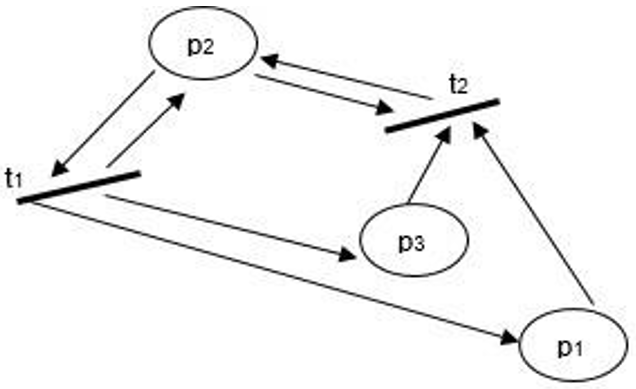
\includegraphics[height=0.2\textheight]{Anexos-07/Imagen1}
	\caption{Red de Petri con marcación inicial $M_0=(0,1,0)$}
	\label{fig:1}
\end{figure}

\begin{enumerate}[a)]
	\item	Indicar los vectores de habilitación y cambio
	\item	Construir el árbol de alcanzabilidad.
	\item	Si se alcanzase el estado $(97,1,97)$, ¿qué transiciones estarían habilitadas y a qué estados se llegaría?.
\end{enumerate}

\subsection{Resultados}

Respecto a la primera actividad, el trabajo realizado por los alumnos fue correcto, en el 100\% de los casos. En la determinación de ambos tipos de vectores hay una generalización implícita alcanzada por los estudiantes, que se presenta en la madurez del uso de la definición de construcción de ambos vectores.

En referencia a la segunda actividad distinguiremos 4 niveles de respuestas: 
\begin{itemize}
	\item \textbf{Nivel 1}: “No realizan la actividad”, responden justificando que ninguna transición está habilitada desde la marcación inicial. Los docentes percibimos en ellos que no han comprendido cuando una transición está habilitada, y es lo primero que se les recomienda revisar y se apoya con nuevos ejercicios para avanzar en el logro de este concepto.
	\item \textbf{Nivel 2}: “Desarrollan sólo tres o cuatro niveles del árbol de alcanzabilidad“ (ver Figura \ref{fig:2}), sin llegar a percibir que hay un proceso de patrones de crecimiento que se podría generalizar por la estructura que poseen los estados alcanzables. Los docentes detectamos que no han iniciado la primera etapa del proceso de generalización de patrones. No han realizado observación crítica, de los resultados que están obteniendo. Sin esa primera etapa indagatoria de la información que se obtiene o posee, no se puede avanzar al descubrimiento de un patrón. Se hace junto a ellos, en sesiones de consulta la deducción de varios niveles más del árbol de alcanzabilidad y mediante preguntas se los guía al descubrimiento de la regularidad. Luego se les plantea un trabajo extra con más ejercitación sobre Redes de Petri con árbol de alcanzabilidad infinito.
	
	\begin{figure}[h]
		\centering
		
\includegraphics[width=0.45\linewidth]{Anexos-07/Imagen2}
		\caption{Respuesta del Nivel 2 de alumnos que no realizan generalización en el árbol de alcanzabilidad.}
		\label{fig:2}
	\end{figure}
	
	\item \textbf{Nivel 3}: “Perciben el patrón pero no realizan la generalización” (ver Figura3). La madurez del proceso de pensamiento los lleva a alcanzar la segunda etapa de la determinación de patrones y luego de una observación exhaustiva de los datos obtenidos pueden responder que sí existe un patrón, pero su proceso inductivo aún es incompleto pues no logran indicar si de esos estados que ahora no están formulados en forma aritmética, habilitan ó no la ejecución de nuevas transiciones, y en caso afirmativo, que forma tendrían los nuevos estados alcanzables. Los docentes debimos volver con estos estudiantes en clases de apoyo, a indagar mediante preguntas dirigidas: a si esos vectores “estados generalizados” tienen disponibles ó no, las marcas necesarias para habilitar alguna/s de las transiciones de la Red?. Haciendo con ello volver a la reflexión de la consulta que nunca se debe olvidar en este tema: cuándo una transición está habilidad, desde un estado?.
	
	\begin{figure}[h]
		\centering
		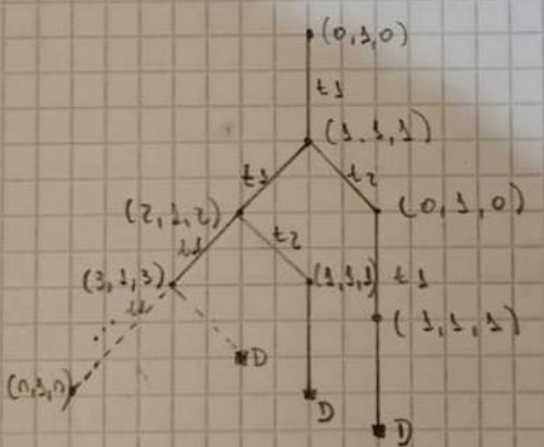
\includegraphics[width=0.45\linewidth]{Anexos-07/Imagen3}
		\caption{Respuesta del Nivel 3 de alumnos que perciben el patrón pero no realizan generalización en el árbol de alcanzabilidad.}
		\label{fig:3}
	\end{figure}
	
	También en este nivel los docentes apoyaron a este grupo de alumnos, con un trabajo extra con más ejercitación sobre Redes de Petri con árbol de alcanzabilidad infinito, en los que se les cuestiona siempre sobre estados con un “muy elevado” número de marcas en los places, con el objeto que no puedan llegar en un desarrollo puntual- a mano alzada, sino que sea fruto de aplicar respuestas de un proceso de generalización.
	
	\item \textbf{Nivel 4}: “Realizan generalización del patrón por aplicación en su razonamiento de método inductivo” (\citet{rivera11}). Su proceso de pensamiento alcanza la etapa de síntesis. Descubriendo a su vez, dentro de este grupo, dos subgrupos: uno que debe pasar en su tarea por muchos casos particulares para llegar a completar la etapa (ver Figura \ref{fig:4}).
	
	\begin{figure}[h]
		\centering
		
\includegraphics[width=0.5\linewidth]{Anexos-07/Imagen4}
		\caption{Respuesta del Nivel 4, primer subgrupo de alumnos que generalizan el patrón, en el árbol de alcanzabilidad.}
		\label{fig:4}
	\end{figure}
	
	El segundo subgrupo que con poco proceso de observación en cada ejercicio que trabaja, puede llegar a la generalización de la regularidad presente en ciertos estados del árbol de alcanzabilidad infinito de la Red de Petri, por aplicación del método inductivo (ver Figura \ref{fig:5}).
	
	\begin{figure}[h]
		\centering
		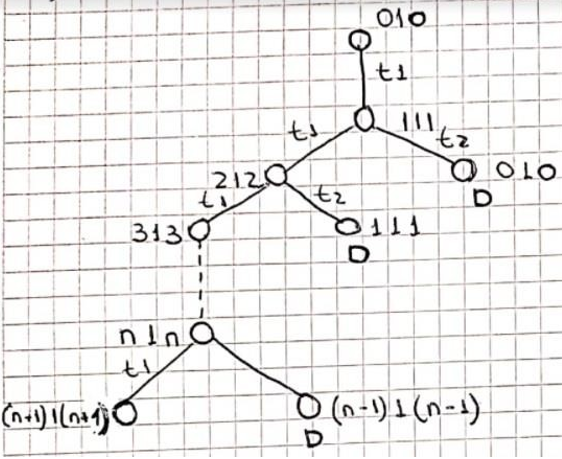
\includegraphics[width=0.5\linewidth]{Anexos-07/Imagen5}
		\caption{Respuesta del Nivel 4, segundo subgrupo de alumnos que generalizan el patrón, en el árbol de alcanzabilidad.}
		\label{fig:5}
	\end{figure}
\end{itemize}

La información de cómo se distribuyeron por niveles, los 80 alumnos (ver Tabla \ref{tab:1}), que son parte de este trabajo.

\begin{table}[h]
	\centering
	\def\arraystretch{1.25}
	\begin{tabular}[h]{|l|c|}
		\hline
		Nivel	&	Número de alumnos\\\hline
		Nivel 1	&	10\\\hline
		Nivel 2	&	34\\\hline
		Nivel 3	&	6\\\hline
		Nivel 4	&	30\\
		\hline
	\end{tabular}
	\caption{Resultados finales de la primera aplicación del proceso}
	\label{tab:1}
\end{table}

Los 50 alumnos que no alcanzaron el Nivel 4, son los que no pudieron responder la tercera actividad. En la recuperación de esta evaluación, se les planteó nuevamente una Red de Petri con árbol de alcanzabilidad infinito, se mantuvieron las dos primeras actividades y se modificó la tercera, por una pregunta sobre a qué estado lleva una secuencia de transiciones ejecutable desde $M_0$, del tipo: (t1)45 t2(t1)30?. Los resultados (ver Tabla \ref{tab:2}) presentan un avance en el logro del contenido.

\begin{table}[h]
	\centering
	\def\arraystretch{1.25}
	\begin{tabular}[h]{|l|c|}
		\hline
		Nivel	&	Número de alumnos\\\hline
		Nivel 1	&	2\\\hline
		Nivel 2	&	3\\\hline
		Nivel 3	&	5\\\hline
		Nivel 4	&	40\\
		\hline
	\end{tabular}
	\caption{Resultados finales de la segunda aplicación del proceso}
	\label{tab:2}
\end{table}

\section{Conclusiones}

Los 30 estudiantes que en el primer proceso de evaluación lograron el Nivel 4, el 80\% de ellos no necesitó la instancia Extraordinaria para regularizar la asignatura. Los 50 estudiantes que en la primer instancia no alcanzaron el Nivel 4, sólo el 36\% de ellos no necesitó la instancia Extraordinaria para regularizar la asignatura; del resto el 28\% quedó libre y el otro 36\% regularizó con uso de la instancia extraordinaria de evaluación.

Los 50 estudiantes que en la primera instancia de evaluación fueron observados en los Niveles 1, 2 y 3, fueron encuestados en un segundo proceso con preguntas concretas sobre análisis específico de estados que les causaron inconvenientes en obtener patrones. Mediante el trabajo guiado en el análisis de casos particulares, pudieron mediante re-observación, arribar a realizar inferencia. La continuidad en el seguimiento en el proceso de aprendizaje permitió superar la dificultad y que el alumno alcanzara autonomía. De este grupo aprobó en la evaluación de recuperación, esta unidad el 80\%.

Esta forma de trabajo con profundo seguimiento de las actividades del alumno, fue adoptada para trabajar este año 2022, pues es la primera experiencia presencial del grupo que cursa la asignatura Matemática Discreta, que son alumnos que cursan su tercer semestre de las carreras Licenciatura en Ciencias de la Computación y Licenciatura en Sistemas de Información.

El método inductivo permite a los estudiantes a realizar trabajos exploratorios, a potenciar la observación, indagación, investigación, y la predicción; permitiendo pronosticar comportamientos y descubrir relaciones: pasos iniciales en la búsqueda de la formalización de patrones en el proceso de generalización.

\section{Bibliografía}

\nocite{*}
\printbibliography

\end{document}